\documentclass{beamer}
\graphicspath{{../graphics/}}
\usepackage{listings}
\usepackage{ulem}
\usepackage{subcaption}
\captionsetup{compatibility=false}
\usepackage[lined,commentsnumbered,linesnumbered]{algorithm2e}
\usepackage{multicol}

\usepackage{xcolor}

\newcommand{\linespace}{\vspace{1em}}

\mode<presentation>
{
  \usetheme{Darmstadt}
  \setbeamertemplate{footline}[frame number]
  \setbeamertemplate{navigation symbols}{}
  \setbeamercovered{transparent}
}

\AtBeginSection[]
{
   \begin{frame}
        \frametitle{Content}
        \tableofcontents[sectionstyle=show/hide,subsectionstyle=show/show/hide]
   \end{frame}
}


\usepackage[utf8]{inputenc}

\usepackage{times}

\usepackage{tikz}
\usetikzlibrary{arrows,calc,positioning,shapes.geometric}

\usepackage{multirow}

\title[OHPAC]{Online Hotspot-based Predictions\\
for Aalborg City Bike}

\subtitle{SW701E14}

\author[SW701E14]{
Mikael Elkiær Christensen \\\and
Alexander Drægert \\\and
Mikkel Sandø Larsen \\\and
Stefan Marstrand Getreuer Micheelsen \\\and
Bruno Thalmann
}

\institute[Aalborg University]
{
  Software\\
  Aalborg University}

\date[CFP 2003]{January 28, 2015}

\begin{document}

% % % % % % % %
% INTRODUCTION
% % % % % % % %

\begin{frame}
  \titlepage
\end{frame}

\begin{frame}
    \frametitle{Content}
    \tableofcontents[sectionstyle=show/show,subsectionstyle=hide/hide/hide]
\end{frame}

% % % % %
% SLIDES
% % % % %

To counter the increasing energy and environmental issues, Aalborg Kommune implemented the CIVITAS-ARCHIMEDES project\cite{aalborgbycyklenbagcyklen}. As part of this project, city bikes were made publicly available for everyday use.
In order to maximize the number of users, the usage was cheap and easy but the bikes were well equipped and was of good quality\cite{cykelplanlaegning}.
To use a bike all you need to do is to place a 20DKK coin into a bike lock. When your ride is over and you lock the bike at the station, you will get your 20DKK back.
\section{Analysis}

\subsection{Aalborg City Bike}

% % % % % %
% Aalborg City Bike as basis
% % % % % %
\begin{frame}
\frametitle{Aalborg City Bike as basis}
\begin{columns}
\begin{column}{.45\textwidth}
\begin{block}{From aalborgbycyklen.dk:}
Take a citybike,
\begin{itemize}
\item when you parked your car and feel like riding along the promenade or harbour.
\item when it's Monday morning and your own bike has a flat tire.
\item when you want to swing by your friends house.
\end{itemize}
\end{block}
\end{column}
\begin{column}{.45\textwidth}
\begin{figure}
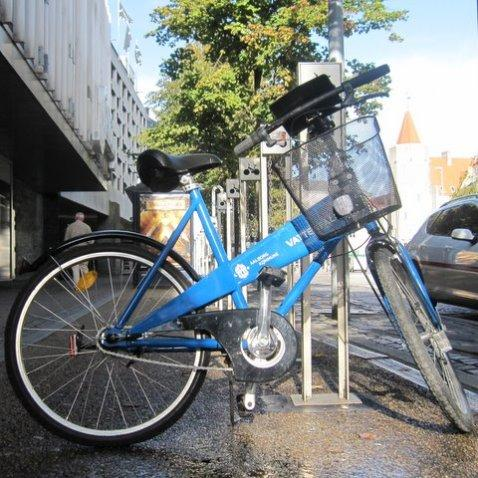
\includegraphics[width=\textwidth]{graphics/acb_bike}
\caption{An Aalborg City Bike (aalborgbycyklen.dk)}
\end{figure}
\end{column}
\end{columns}
\end{frame}

% % % % % %
% Aalborg City Bike facts
% % % % % %
\begin{frame}
\frametitle{Aalborg City Bike facts}
\begin{columns}
\begin{column}{.44\textwidth}
\begin{itemize}
\item 200 bikes
\begin{itemize}
\item 140 active
\end{itemize}
\item 21 bike stations
\begin{itemize}
\item Room for 170 bikes
\end{itemize}
\item Each bike has a lock, attached to a station
\item Unlock with 20 DKK coin, re-locking returns the coin
\end{itemize}
\end{column}
\begin{column}{.44\textwidth}
\begin{figure}
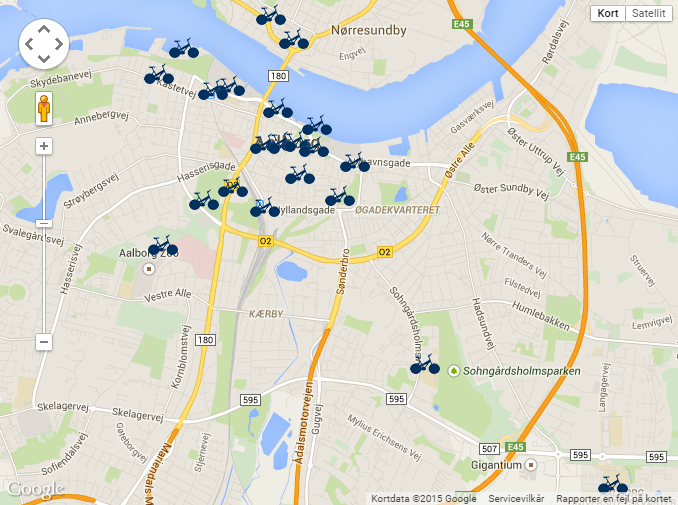
\includegraphics[width=\textwidth]{graphics/acb_gmaps}
\caption{Map of all bike stations in Aalborg/Nørresundby Area (aalborgbycyklen.dk)}
\end{figure}
\end{column}
\end{columns}
\end{frame}

% % % % % %
% Interview and existing systems
% % % % % %
\begin{frame}
\frametitle{Interview and existing systems}
{\Huge ?}
\end{frame}

% % % % % %
% Analysis summary
% % % % % %
\begin{frame}
\frametitle{Analysis summary}
\begin{columns}
\begin{column}{.45\textwidth}
\begin{block}{Problems\footnotemark}
\begin{enumerate}
\item Bikes left outside stations
\item Too few stations
\item Making short stops
\item No bikes at station
\item No way of knowing when a bike will arrive
\item Broken bikes
\end{enumerate}
\end{block}
\end{column}
\begin{column}{.45\textwidth}
\begin{block}{Limitations/requests\footnotemark[1]}
\begin{enumerate}
\item No renting/booking system
\item No specific target user group
\item Interested in statistics about usage
\item Short period usage
\end{enumerate}
\end{block}
\end{column}
\end{columns}
\footnotetext{Section 1.4.1, p. 10}
\end{frame}

\subsection{Problem statement}

% % % % % %
% Trivially solved
% % % % % %
\begin{frame}
\frametitle{Trivially solved}
\begin{block}{Problems}
\begin{enumerate}
\item \textbf{Bikes left outside stations}
\item \textbf{Too few stations}
\item \textbf{Making short stops}
\item \textbf{No bikes at station}
\item No way of knowing when a bike will arrive
\item \textbf{Broken bikes}
\end{enumerate}
\end{block}
\end{frame}

% % % % % %
% New problems
% % % % % %
\begin{frame}
\frametitle{New problems}
\begin{enumerate}
\item Defining and identifying hotspots
\item Modelling the usage and using the model for predictions
\item Making the data available through a web service
\end{enumerate}
\end{frame}

% % % % % %
% Solution
% % % % % %
\begin{frame}
\frametitle{Solution}

\centering
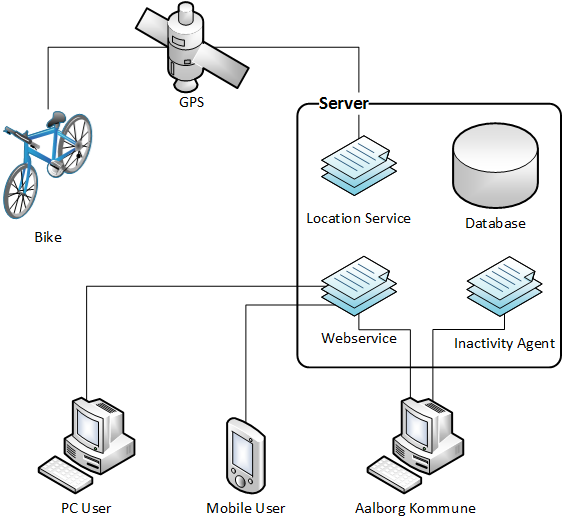
\includegraphics[height=.9\textheight]{our_solution}

\end{frame}
\section{Finding Hotspots}

\subsection{Clustering}
\subsubsection{General}
\subsubsection{Data}
\subsubsection{Noise}
\begin{frame}
\frametitle{General}
	\begin{itemize}
		\item Because ...
	\end{itemize}
\end{frame}	
\begin{frame}
\frametitle{Data}
	\begin{center}
		%Make better example picture with standards from program.
		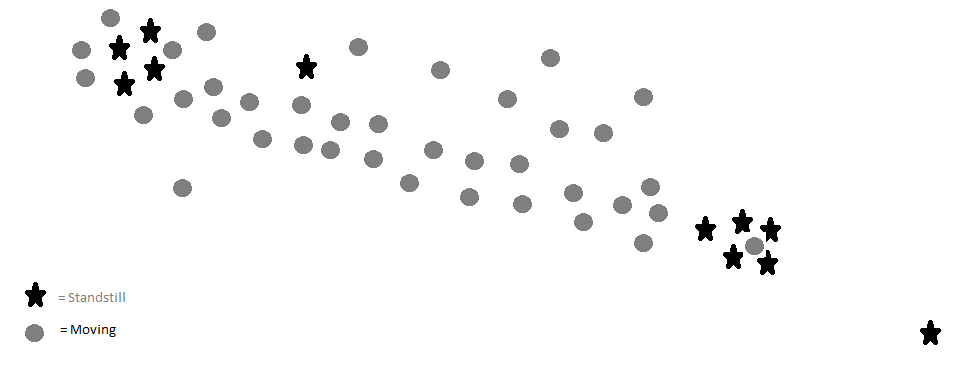
\includegraphics[scale=0.5]{graphics/pointtype-example}
	\end{center}
\end{frame}	
\begin{frame}
\frametitle{Noise}
	\begin{center}
		%Make example picture with noise points.
		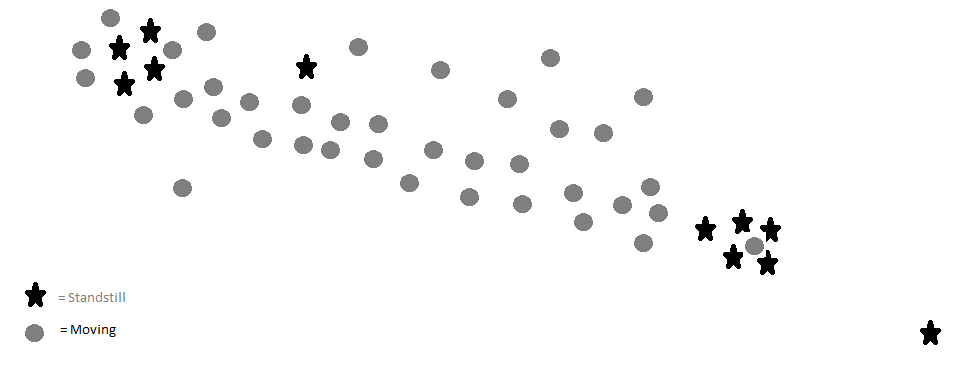
\includegraphics[scale=0.5]{graphics/pointtype-example}
	\end{center}
\end{frame}	

\subsubsection{DBSCAN} %Partial Clustering? - from presentation notes.
\begin{frame}
\frametitle{Expected data}
	\begin{itemize}
		\item Partitional - No need for hierarchies.
		\item Exclusive - Separated clusters.
		\item Partial - Need for expected outliers.
		\item Density based - The number of data points is important.
	\end{itemize}
\end{frame}	
\begin{frame}
\frametitle{DBSCAN Parameters}
	\begin{itemize}
		\item DBSCAN ...
	\end{itemize}
\end{frame}	

%Slide med de 2 parameter og hvordan vi sætter dem. Hvad de betyder etc.

\subsection{Convex Hull}
\subsubsection{How does Convex Hull work?}
\subsubsection{Other reduction strategies}
\begin{frame}
\frametitle{Other reduction strategies - Rectangle}
\begin{multicols}{2}
	\begin{itemize}
		\item Advantages:
		\begin{itemize}
			\item Property ...
		\end{itemize}
		\item Disadvantages:
		\begin{itemize}
			\item Property ...
		\end{itemize}
	\end{itemize}
\columnbreak
	\begin{center}
		%Images of Convex Hull vs Square
		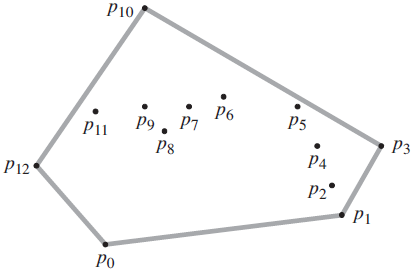
\includegraphics[scale=0.5]{graphics/convexHull-example}\\
		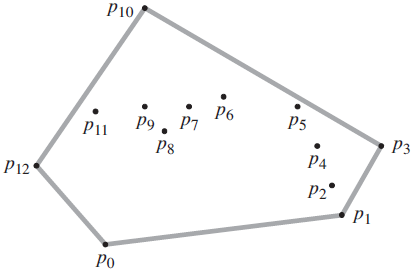
\includegraphics[scale=0.5]{graphics/convexHull-example}
	\end{center}
\end{multicols}
\end{frame}
\begin{frame}
\frametitle{Other reduction strategies - Circle/Elipse}
\begin{multicols}{2}
	\begin{itemize}
		\item Advantages:
		\begin{itemize}
			\item Property ...
		\end{itemize}
		\item Disadvantages:
		\begin{itemize}
			\item Property ...
		\end{itemize}
	\end{itemize}
\columnbreak
	\begin{center}
		%Images of Convex Hull vs Circle
		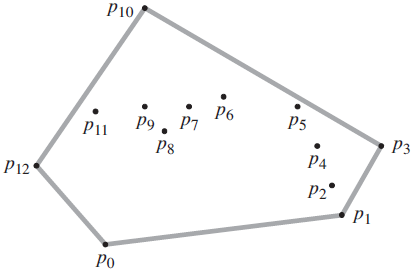
\includegraphics[scale=0.5]{graphics/convexHull-example}\\
		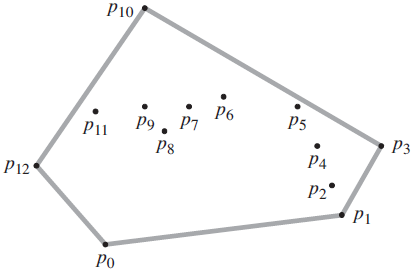
\includegraphics[scale=0.5]{graphics/convexHull-example}
	\end{center}
\end{multicols}
\end{frame}	
\begin{frame}
\frametitle{Other reduction strategies - Polygon}
\begin{multicols}{2}
	\begin{itemize}
		\item Advantages:
		\begin{itemize}
			\item Property ...
		\end{itemize}
		\item Disadvantages:
		\begin{itemize}
			\item Property ...
		\end{itemize}
	\end{itemize}
\columnbreak
	\begin{center}
		%Images of Convex Hull vs Polygon
		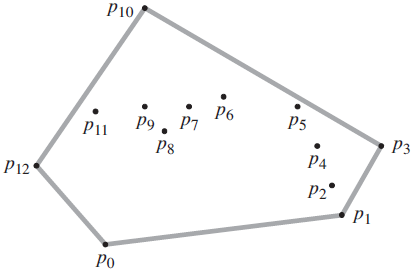
\includegraphics[scale=0.5]{graphics/convexHull-example}\\
		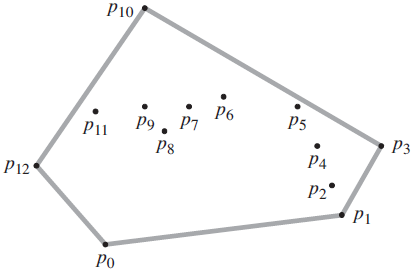
\includegraphics[scale=0.5]{graphics/convexHull-example}
	\end{center}
\end{multicols}
\end{frame}
\begin{frame}
\frametitle{How does Convex Hull work?}
\begin{multicols}{2}
	\begin{itemize}
		\item Advantages:
		\begin{itemize}
			\item Property ...
		\end{itemize}
		\item Disadvantages:
		\begin{itemize}
			\item Property ...
		\end{itemize}
	\end{itemize}
\columnbreak
	\begin{center}
		%Images of Convex Hull vs Polygon
		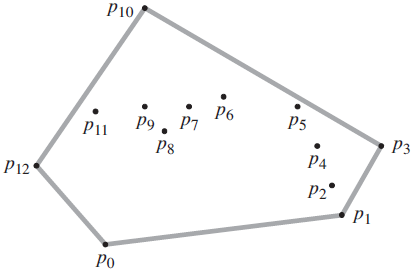
\includegraphics[scale=0.5]{graphics/convexHull-example}\\
		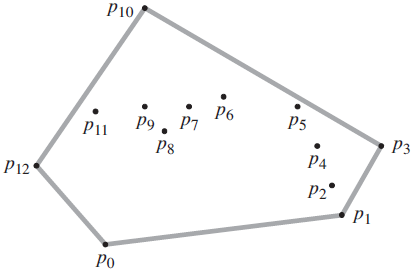
\includegraphics[scale=0.5]{graphics/convexHull-example}
	\end{center}
\end{multicols}
\end{frame}
\section{Predicting Behaviour}
\begin{frame}{The prediction problem}
\begin{center}
How much time will it take before a bike will be \emph{in a given hotspot}

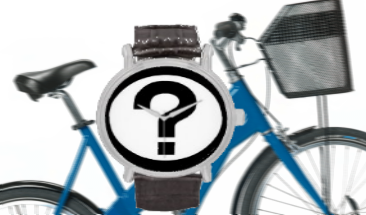
\includegraphics[width=0.8\linewidth]{graphics/biketime}
\end{center}

\end{frame}

\subsection{Modeling the system}

\begin{frame}{Simple hotspot model}
\begin{center}
\begin{figure}[H]
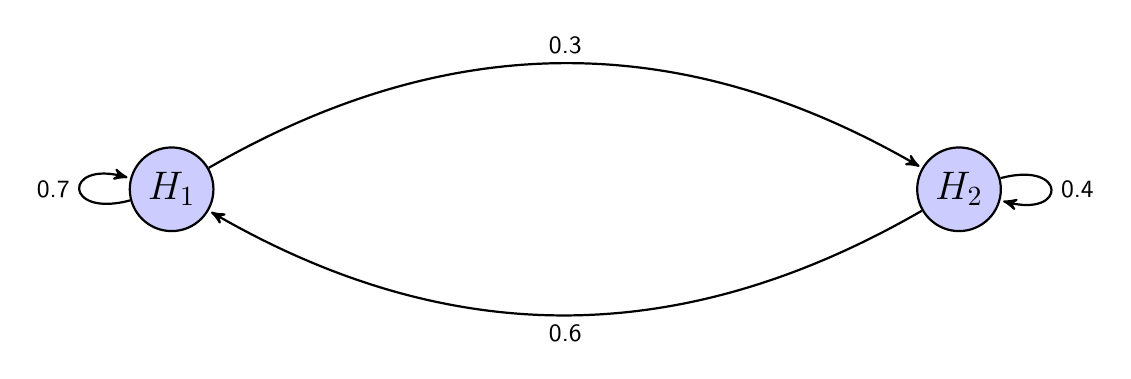
\begin{tikzpicture}[->,>=stealth',shorten >=1pt,auto,node distance=10cm,
  thick,main node/.style={circle,fill=blue!20,draw,font=\sffamily\Large\bfseries}]

  \node[main node] (1) {$H_1$};
  \node[main node] (2) [right of=1] {$H_2$};

  \path[every node/.style={font=\sffamily\small}]
    (1) edge [bend left] node {0.3} (2)
        edge [loop left] node {0.7} (1)
    (2) edge [bend left] node {0.6} (1)
        edge [loop right] node {0.4} (2);
\end{tikzpicture}
\caption{A Markov chain model of a system with two bike hotspots}
\label{markov:model:simple}
\end{figure}

\begin{itemize}
	\item Discrete time markov chain
	\item States represent hotspots
	\item Time- homogeneous
\end{itemize}
\end{center}
\end{frame}

\begin{frame}
\begin{center}
Where do we place the black bike?	
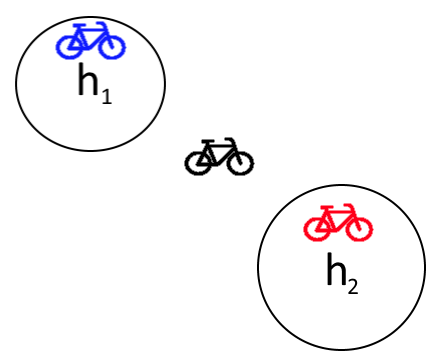
\includegraphics[scale=0.7]{graphics/world}
\end{center}
\end{frame}

\begin{frame}{Departure state model}
\begin{figure}[h]
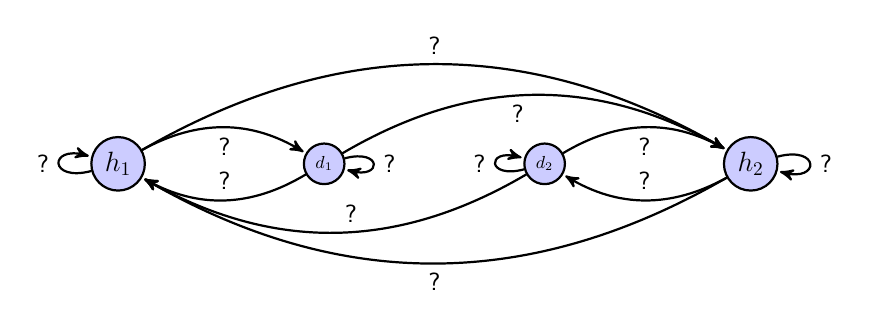
\begin{tikzpicture}[->,>=stealth',shorten >=1pt,auto,node distance=4cm,
  thick,main node/.style={circle,fill=blue!20,draw,font=\sffamily\Large\bfseries},every node/.style={scale=0.7}]

  \node[main node] (B1) {$h_1$};
  \node[main node,font=\sffamily\small] (D1) [right = 2cm of B1] {$d_1$};
  \node[main node,font=\sffamily\small] (D2) [right of=D1] {$d_2$};
  \node[main node] (B2) [right = 2cm of D2] {$h_2$};

  \path[every node/.style={font=\sffamily\small}]
    (B1) edge [bend left] node {?} (B2)
         edge [loop left] node {?} (B1)
         edge [bend left] node[below] {?} (D1)
    (B2) edge [bend left] node {?} (B1)
         edge [loop right] node {?} (B2)
         edge [bend left] node[above] {?} (D2)
    (D1) edge [bend left] node[above] {?} (B1)
         edge [loop right] node {?} (D1)
         edge [bend left] node[below left] {?} (B2)
    (D2) edge [bend left] node[below] {?} (B2)
         edge [loop left] node {?} (D2)
         edge [bend left] node[above right] {?} (B1);
\end{tikzpicture}
\end{figure}

% VISUALIZE
% http://setosa.io/blog/2014/07/26/markov-chains/index.html
%[[0.65,0.30,0.05,0.00],
%[0.10,0.60,0.30,0.00],
%[0.15,0.00,0.50,0.35],
%[0.20,0.00,0.10,0.70]
%]
\end{frame}

\subsection{Creating the model}

\begin{frame}{}
	
\begin{center}
We want to generate the model with data from the GPS receivers on the bikes
	
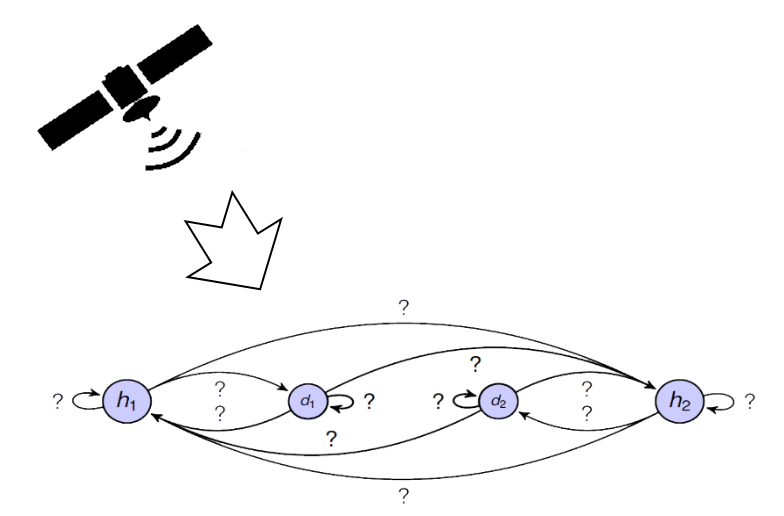
\includegraphics[width=0.8\linewidth]{graphics/build_the_model}
\end{center}

\end{frame}

\begin{frame}{Locate the bike}
	
t=0

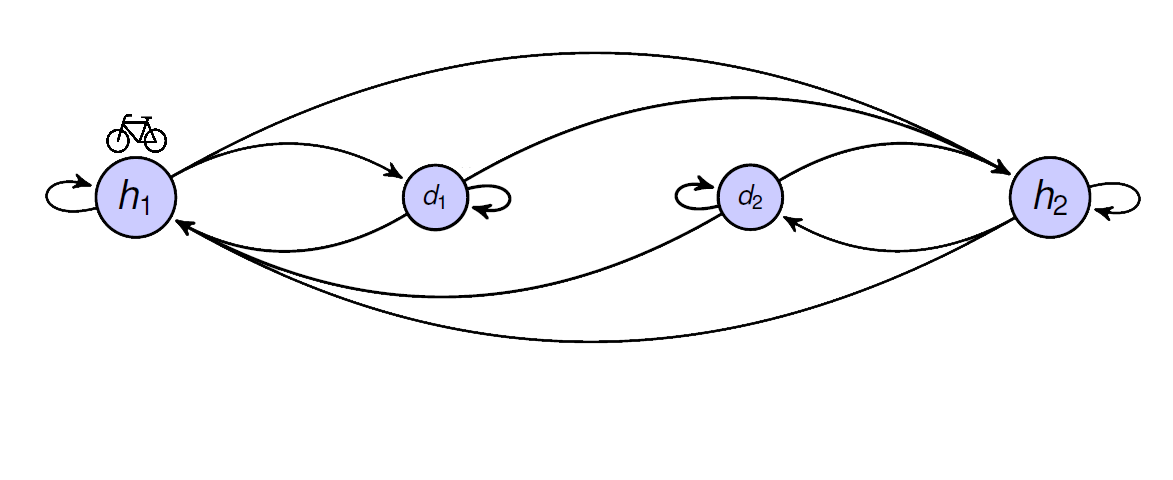
\includegraphics[width=\linewidth]{graphics/createmarkov_initial}
\[
\kbordermatrix{ 
	&  h_1 &  d_1  &  h_2  &  d_2 \\
	h_1  & 0 & 0 & 0 & 0\\
	d_1 & 0  & 0 & 0  & 0\\
	h_2  & 0 & 0   & 0 & 0\\
	d_2  & 0  & 0   & 0  & 0
}
\]
	
\end{frame}

\begin{frame}{Track the route of the bike}
t=1	
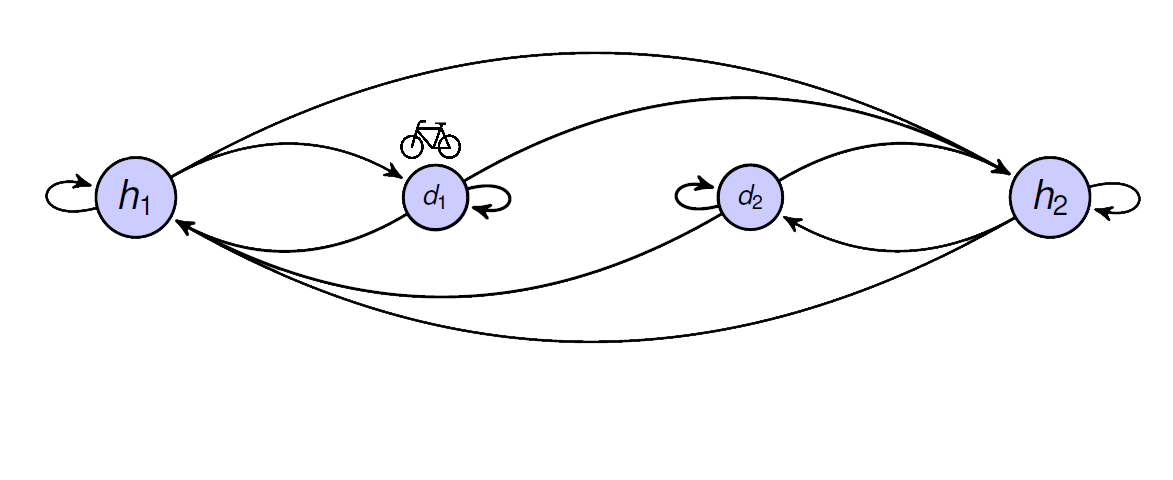
\includegraphics[width=\linewidth]{graphics/createmarkov_firststep}	
\[
	\kbordermatrix{ 
		&  h_1 &  d_1  &  h_2  &  d_2 \\
		h_1  & 0 & 1 & 0 & 0\\
		d_1 & 0  & 0 & 0  & 0\\
		h_2  & 0 & 0   & 0 & 0\\
		d_2  & 0  & 0   & 0  & 0
	}
	\]
	
\end{frame}

\begin{frame}{Track the route of the bike}
t=4
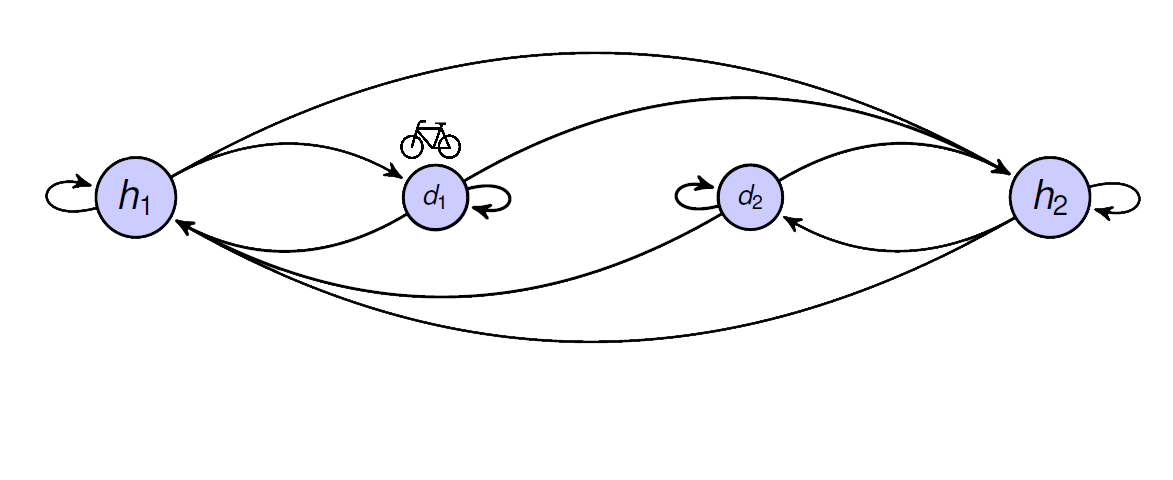
\includegraphics[width=\linewidth]{graphics/createmarkov_firststep}		
\[
	\kbordermatrix{ 
	&  h_1 &  d_1  &  h_2  &  d_2 \\
	h_1  &  0& 1 & 0 & 0\\
	d_1 & 0  & 3 & 0  & 0\\
	h_2  & 0 & 0   & 0 & 0\\
	d_2  & 0  & 0   & 0  & 0
}
\]	
\end{frame}

\begin{frame}{Track the route of the bike}
	t=5
	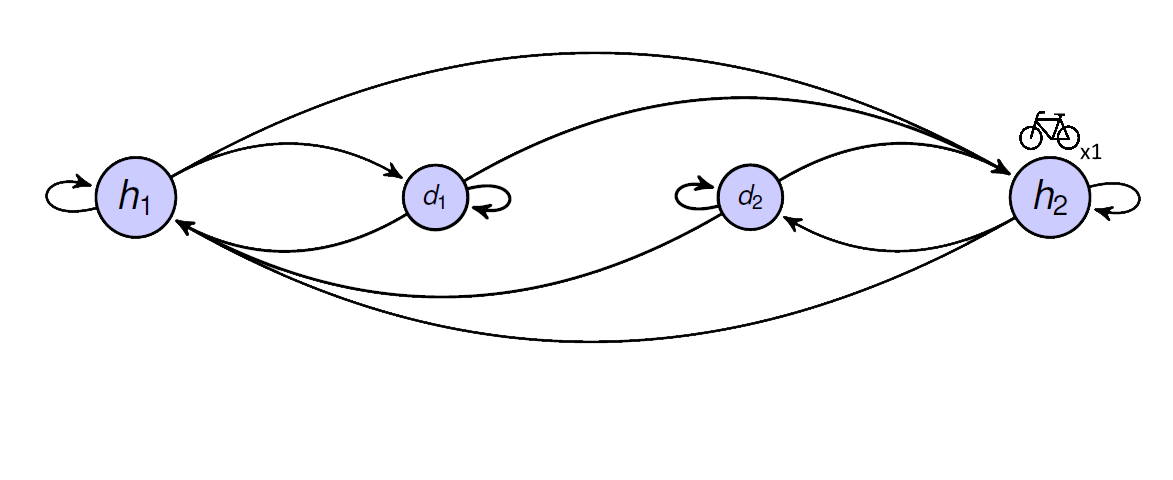
\includegraphics[width=\linewidth]{graphics/createmarkov_laststep}		
	\[
	\kbordermatrix{ 
		&  h_1 &  d_1  &  h_2  &  d_2 \\
		h_1  &  0& 1 & 0 & 0\\
		d_1 & 0  & 3 & 1  & 0\\
		h_2  & 0 & 0   & 0 & 0\\
		d_2  & 0  & 0   & 0  & 0
	}
	\]	
\end{frame}


\begin{frame}{Complete for all bikes}
t=$ t_n $
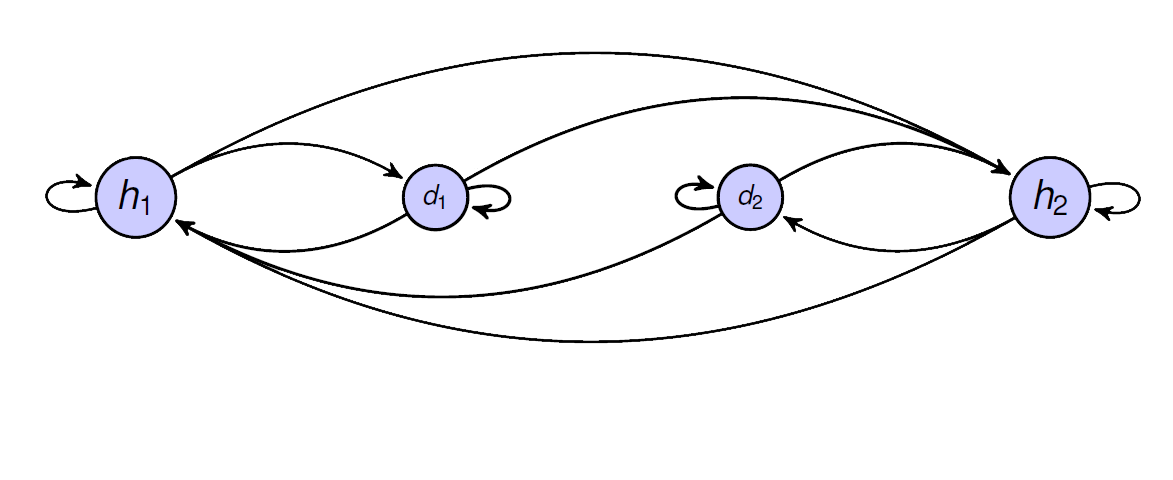
\includegraphics[width=\linewidth]{graphics/createmarkov_final}	
	\[
	\kbordermatrix{ 
		&  h_1 &  d_1  &  h_2  &  d_2 \\
		h_1  & 13 & 6 & 2 & 0\\
		d_1 & 2  & 12 & 6  & 0\\
		h_2  & 3 & 0   & 7 & 10\\
		d_2  &  4 & 0   & 2  & 14
	}
	\]		
	
\end{frame}

\begin{frame}[fragile]{Normalize the matrix}
\begin{figure}[H]
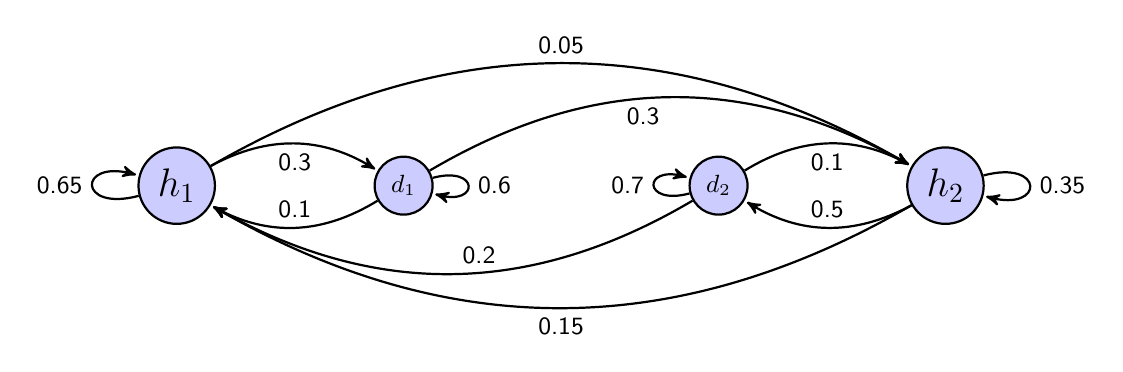
\begin{tikzpicture}[->,>=stealth',shorten >=1pt,auto,node distance=4cm,
  thick,main node/.style={circle,fill=blue!20,draw,font=\sffamily\Large\bfseries}]

  \node[main node] (B1) {$h_1$};
  \node[main node,font=\sffamily\small] (D1) [right = 2cm of B1] {$d_1$};
  \node[main node,font=\sffamily\small] (D2) [right of=D1] {$d_2$};
  \node[main node] (B2) [right = 2cm of D2] {$h_2$};

  \path[every node/.style={font=\sffamily\small}]
    (B1) edge [bend left] node {0.05} (B2)
         edge [loop left] node {0.65} (B1)
         edge [bend left] node[below] {0.3} (D1)
    (B2) edge [bend left] node {0.15} (B1)
         edge [loop right] node {0.35} (B2)
         edge [bend left] node[above] {0.5} (D2)
    (D1) edge [bend left] node[above] {0.1} (B1)
         edge [loop right] node {0.6} (D1)
         edge [bend left] node[below left] {0.3} (B2)
    (D2) edge [bend left] node[below] {0.1} (B2)
         edge [loop left] node {0.7} (D2)
         edge [bend left] node[above right] {0.2} (B1);
\end{tikzpicture}
\caption{A Markov chain model with two hotspots and departure states}
\label{markov:model:complex}
\end{figure}

% VISUALIZE
% http://setosa.io/blog/2014/07/26/markov-chains/index.html
%[[0.65,0.30,0.05,0.00],
%[0.10,0.60,0.30,0.00],
%[0.15,0.00,0.50,0.35],
%[0.20,0.00,0.10,0.70]
%]
\[
\kbordermatrix{ 
	&  h_1 &  d_1  &  h_2  &  d_2 \\
	h_1  & 0.65 & 0.3 & 0.05 & 0\\
	d_1 & 0.1  & 0.6 & 0.3  & 0\\
	h_2  & 0.15 & 0   & 0.35 & 0.5\\
	d_2  & 0.2  & 0   & 0.1  & 0.7
}
\]		

\end{frame}




\subsection{Predicting with the model}

\begin{frame}{Find the initial distribution}
\begin{center}

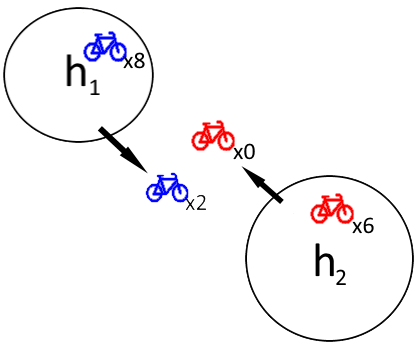
\includegraphics[scale=0.7]{graphics/initialworld2}
	
$(
\underset{h_1}{8},
\underset{d_1}{2},
\underset{h_2}{6},
\underset{d_2}{0}
)$
\end{center}
\end{frame}

\begin{frame}[fragile]
	

	
\begin{center}	
	
$ P_i \times \tau_M = P_{i+1}$\\

\begin{itemize}
	\item \textbf{$ P_i $} - bike distribution at time $ i $
	\item \textbf{$ \tau_M $} - the markov transition function 
\end{itemize}
		
		

\[
(\underset{h_1}{8},
\underset{d_1}{2},
\underset{h_2}{6},
\underset{d_2}{0})	
\begin{bmatrix}
0.65 & 0.3 & 0.05 & 0\\
0.1  & 0.6 & 0.3  & 0\\
0.15 & 0   & 0.35 & 0.5\\
0.2  & 0   & 0.1  & 0.7
\end{bmatrix}
=
(
\underset{h_1}{6.3},
\underset{d_1}{3.6},
\underset{h_2}{3.1},
\underset{d_2}{3}
)
\]

\[
(
\underset{h_1}{6.3},
\underset{d_1}{3.6},
\underset{h_2}{3.1},
\underset{d_2}{3}
)
\begin{bmatrix}
0.65 & 0.3 & 0.05 & 0\\
0.1  & 0.6 & 0.3  & 0\\
0.15 & 0   & 0.35 & 0.5\\
0.2  & 0   & 0.1  & 0.7
\end{bmatrix}
=
(
\underset{h_1}{5.52},
\underset{d_1}{4.05},
\underset{h_2}{2.78},
\underset{d_2}{3.65}
)
\]


\end{center}
\end{frame}

\begin{frame}{Predicting with accumulation}
Simulating that bikes never leave the hotspot where the user is waiting

$$ \begin{bmatrix}
	{\color{red}1} & {\color{blue}0} & \color{blue} 0& {\color{blue}0}\\
	0.1  & 0.6 & 0.3  & 0\\
	0.15 & 0   & 0.35 & 0.5\\
	0.2  & 0   & 0.1  & 0.7
\end{bmatrix}
 $$
\end{frame}


\begin{frame}{Two steps of accumulation}
$$
(8, 2, 6, 0)
\begin{bmatrix}
1 & 0 & 0 & 0\\
0.1  & 0.6 & 0.3  & 0\\
0.15 & 0   & 0.35 & 0.5\\
0.2  & 0   & 0.1  & 0.7
\end{bmatrix}
=
(9.1,1.2,2.7,3)
$$
	
$$
(9.1,1.2,2.7,3)
\begin{bmatrix}
1 & 0 & 0 & 0\\
0.1  & 0.6 & 0.3  & 0\\
0.15 & 0   & 0.35 & 0.5\\
0.2  & 0   & 0.1  & 0.7
\end{bmatrix}
=
(10.225,0.72,1.605,3.45)
$$
	
\end{frame}

\begin{frame}{Comparison}
	
		Without accumulation
		$$
		(8,2,6,0)
		{\begin{bmatrix}
		0.65 & 0.3 & 0.05 & 0\\
		0.1  & 0.6 & 0.3  & 0\\
		0.15 & 0   & 0.35 & 0.5\\
		0.2  & 0   & 0.1  & 0.7
		\end{bmatrix}}^2
		=
		(5.52,4.05,2.78,3.65)
		$$
		
		With accumulation
$$
(8,2,6,0)
{\begin{bmatrix}
1 & 0 & 0 & 0\\
0.1  & 0.6 & 0.3  & 0\\
0.15 & 0   & 0.35 & 0.5\\
0.2  & 0   & 0.1  & 0.7
\end{bmatrix}}^2
=
(10.225,0.72,1.605,3.45)
$$
	
\end{frame}

\section{Demo}
\subsection{Simulation}

\begin{frame}
\frametitle{Configuration}
\begin{itemize}
\item A system where locations are retrieved from GPS receivers.
\item There is no such system yet.
\item Simulate such a system:
\begin{itemize}
\item $\pm$30 seconds delay from the GPS receiver.
\item The GPS Data is perturbed.
\item Lost GPS Data is not taken into account.
\end{itemize}
\end{itemize}
\end{frame}

\begin{frame}
\frametitle{Setup}
\begin{itemize}
\item 5 bikes.
\item 3 addresses.
\item The BikeVisualizer shows us the GPS data and how they are interpreted.
\end{itemize}
\end{frame}



\section{Conclusion}


\end{document}